\documentclass[10pt]{beamer}
\usepackage[utf8]{inputenc}
\usepackage[T1]{fontenc}
\usepackage{lmodern}
\usepackage[french]{babel}
\usetheme{Frankfurt}

\usepackage{geometry}
\usepackage{keyval, listings}
\lstloadlanguages{[Ansi]C++, Java}


\usepackage{amsfonts, amstext, array, boxedminipage, %
	ifthen, fancybox, multirow, fancyhdr, pgf, tikz%
}
%epsfig, psfrag, , %pstricks,pst-plot,pst-math,pst-infixplot}

%\usepackage{xypic}

\usepackage{caption}
\usepackage{hyperref}

\usepackage{wrapfig}
\usepackage{subfig}

\definecolor{gray}{rgb}{0.95,0.95,0.95}
% Mise au point de l'environnement pour le code
\lstnewenvironment{code}
{\lstset{language=[Ansi]C++,basicstyle=\normalsize\tt,%
		keywordstyle=\ttfamily\bfseries\underbar,%
		commentstyle=\normalsize, extendedchars=true, fontadjust=true, columns = flexible, flexiblecolumns=true,
		linewidth=.975\linewidth, backgroundcolor=\color{gray}, frame=tlrb, xleftmargin=1cm}
	}%, framexleftmargin=5mm,frame=box}}
{}

\begin{document}
	\author{Hakim Ferrier-Belhaouari}
	\title{M1 INFO IHM - Introduction à Unity}
	%\subtitle{}
	%\logo{}
	%\institute{}
	%\date{}
	%\subject{}
	%\setbeamercovered{transparent}
	%\setbeamertemplate{navigation symbols}{}
	\begin{frame}[plain]
		\maketitle
	\end{frame}

	
\section{Introduction}

%\url{https://docs.unity3d.com/}

% \subsection{Introduction}
\begin{frame}[fragile]{Les moteurs de jeu vidéo}  
  
  \begin{block}{Inclus des moteurs}
    \begin{itemize}
    \item graphique 3D
    \item graphique 2D
    \item physique
    \item audio (2D/3D)
    \item réseau
    \item intelligence artificielle (pathfinding, \ldots)
    \item animation
    \item \ldots
    \end{itemize}
  \end{block}

\begin{alertblock}{En bref}
\begin{itemize}
	\item C'est compliqué car mêle beaucoup de spécialité.
	\item Au final, nous avons une boucle perpétuelle de mise à jour de l'image produite et de l'animation d'une \textit{frame}.
\end{itemize}	
\end{alertblock}

\end{frame}


\begin{frame}{Unity}
\begin{block}{C'est quoi?}
	Unity est un \textbf{moteur de jeu multiplateformes} pour les jeux vidéos sous la forme d'un \textbf{environnement de développement intégré}. 
	
%	Il rend la création de jeu beaucoup plus facile en intégrant toutes les complexités et en offrant une utilisation plausible pour les non-experts.
\end{block}

\begin{block}{Historique}
\begin{itemize}
	\item 2000: Création des prémisses d'Unity par 3 danois: volonté de mettre en avant leur expertise.
	\item 2004: Fondation de Unity Technologies à San Francisco.
	\item 2005: première version de Unity (double licences).
	\item 2009: ajout de Direct3D.
	\item 2010: création de l'Asset Store (achat d'objet ou autre).
	\item 2011: achat de Mecanim: ajout d'animations simples directement dans Unity + ajout de DirectX 11.
	\item 2013: ajout d'optimisation des jeux 2D pour répondre à la demande.
	\item 2015: intégration de NVIDIA PhysX.
	\item 2017: intégration un rendu graphique temps réel.
\end{itemize}
\end{block}

\end{frame}

\begin{frame}{Versions}
	\begin{block}{Succès pour des raisons économiques}
% TODO: \usepackage{graphicx} required
\begin{center}
	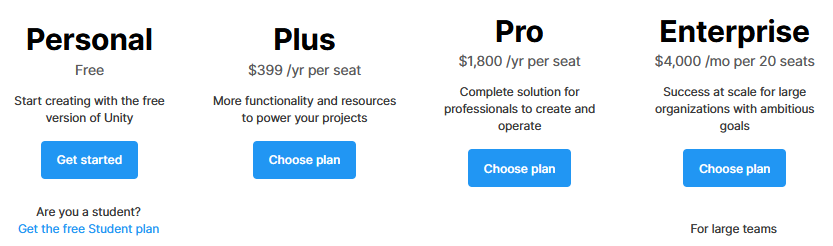
\includegraphics[width=0.5\linewidth]{../../imgs/licence_plan}
\end{center}

	La version personnelle est amplement suffisante pour ce cours, car fonctionne sous les plateformes classiques.
	\end{block}

	\begin{block}{Mécanisme de HUB (version cours: \texttt{6000.0.XXX} chez vous (on verra en TP))}
\begin{center}
\hfill
	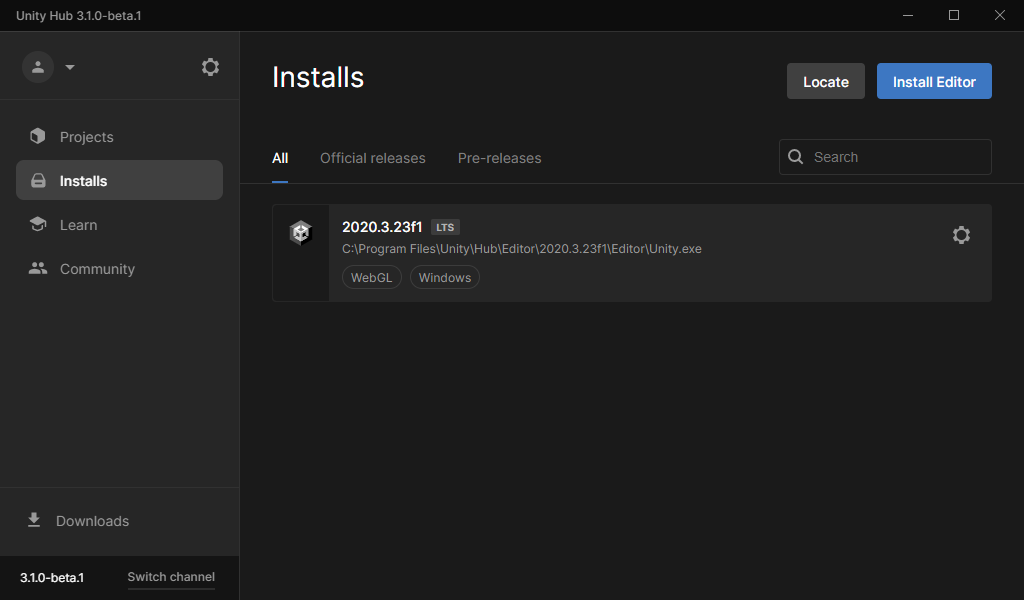
\includegraphics[width=0.45\linewidth]{../../imgs/unity_hub}
\hfill
	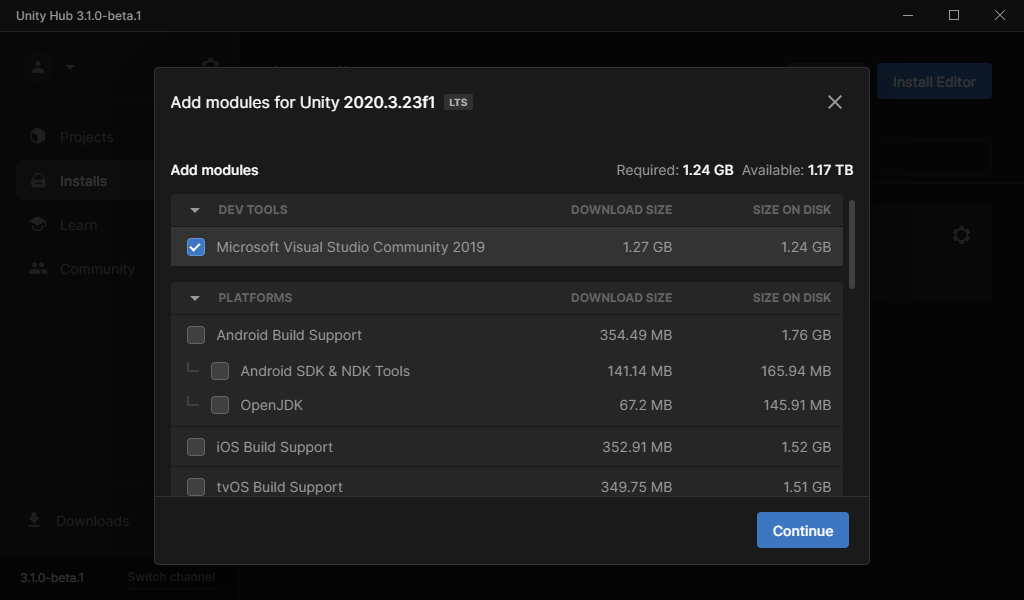
\includegraphics[width=0.45\linewidth]{../../imgs/unity_hub_module}
\hfill
\end{center}

	\end{block}
\end{frame}

\section{Lancement d'Unity}

\begin{frame}{Lancement d'Unity}
\begin{center}
	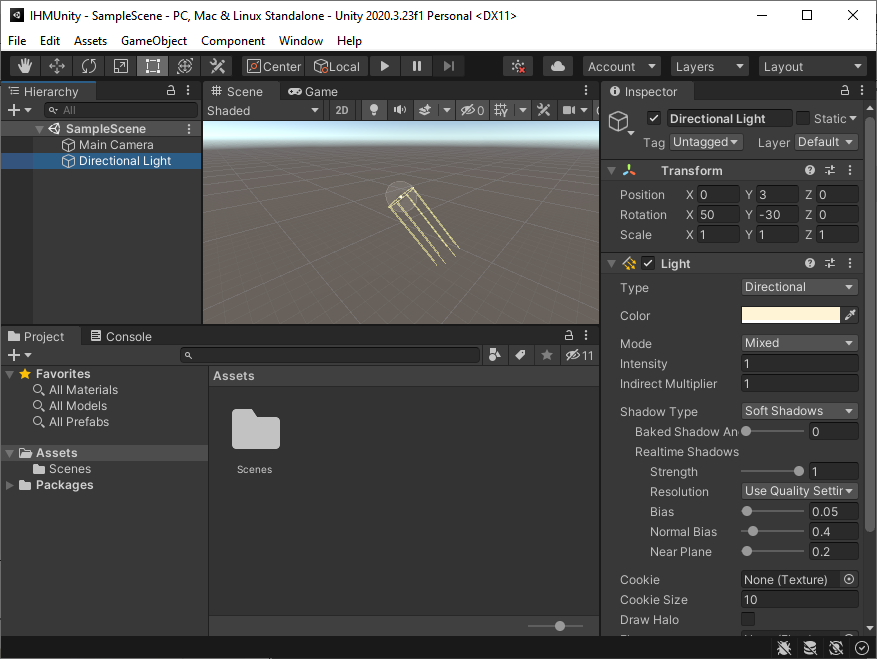
\includegraphics[width=1\linewidth]{../../imgs/interface_basique}
\end{center}

\end{frame}

\begin{frame}{Lancement d'Unity}
	Les onglets sont importants et en voici les principaux:
\begin{enumerate}
	\item Hierarchy: donne une vue sous forme d'arbre de la zone 3D et des objets présents dans votre \texttt{scène}( = correspond à un niveau de votre jeu) ou vos scènes.
	\item Scene: présente la vue 3D de la scène en cours.
	 \item Game: vu de votre application quand vous l'exécutez en direct.
	 \item Inspector: donne l'ensemble des propriétés de votre sélection.
	 \item Project: permet d'explorer l'entièreté de votre projet (dont les Assets)
	 \item Console: donne tous les messages de log de Unity.
\end{enumerate}	

~\\

La barre de lancement 

\includegraphics[width=0.1\linewidth]{../../imgs/unity_barre_lancement}

\begin{enumerate}
	\item lance l'execution de votre application directement. Et arrête son exécution aussi.
	\item met en pause l'exécution (pratique pour déboguer).
	\item et le bouton step toujours pour le débogage.
\end{enumerate}
\end{frame}

\begin{frame}{Demo1}
	\vfill
	\begin{block}{Objectifs}
	\begin{itemize}
		\item Créez un projet 3D nommé \texttt{IHMUnity\_Demo1}.
		\item Regardez les paramètres de votre application (Project Settings > Player)
		\item Ajoutez des objets primitives (1 cube et 1 sphère) dans la vue 3D.
		\item Regardez leurs propriétés et repérez les similitudes et différences.
		\item Lancez l'exécution de la vue.
		\item Pourquoi rien ne se passe?
		\item Modifier la position du cube en direct sans arrêter la simulation.
		\item Stopper la simulation.
		\item Que remarquez vous sur les positions?
	\end{itemize}
	\end{block}
	\vfill
\end{frame}

\section{La classe GameObject en Unity}

\begin{frame}{La classe GameObject}
	
	\begin{definition}
		La classe \textbf{GameObject} est la classe de base de tous les objets présents dans une scène. Leur spécificité est la notion de composant (\textbf{Component}).
	\end{definition}

	\begin{exampleblock}{Exemple: Transform}
		Le composant Transform gère le position de l'objet dans la scène.
	\end{exampleblock}

	\begin{exampleblock}{Exemple: MeshFilter}
	Le composant MeshFilter gère le maillage de l'objet.
\end{exampleblock}

\begin{alertblock}{Les composants}
	Les composants représentent le c\oe ur de la programmation en Unity. Ainsi, pour un objet il suffit de lui ajouter le bon composant pour lui modifier/influencer/ajouter un comportement ou une mécanique.
	
	Lorsqu'il n'y a pas de composant adéquat à votre besoin il nous suffit de le \alert{programmer}!
\end{alertblock}
	
\end{frame}

\begin{frame}{Demo2}
		\vfill
	\begin{block}{Objectifs}
		Sur le projet précédent:
		\begin{itemize}
			\item Ajoutez un composant système de particule au cube.
			\item Amusez vous pour voir les modifications induits en simulation.
			\item Stoppez tout.
			\item Ajoutez un objet 3D Quad, plane ou cube.
			\item Ajoutez un composant vidéo.
			\item Lancez la simulation pour voir l'animation de la vidéo sur l'objet.
			\item Stopper la simulation.
			\item Que remarquez vous sur les positions?
		\end{itemize}
	\end{block}
	\vfill
\end{frame}

\section{Composant Script en Unity}

\begin{frame}[fragile]{Composant script}
	\begin{block}{Prélude}
		Comme nous allons devoir coder, donc réflexes de développeur:
		\begin{itemize}
			\item Préparation de la documentation officielle: \url{https://docs.unity3d.com/}. Cette dernière se décompose en un manuel d'utilisation (guide) et d'une référence technique (Scripting API).
			\item La référence technique montre 2 espaces de noms distincts:
			\begin{enumerate}
				\item UnityEngine: qui contient l'ensemble des fonctionnalités accessible à l'exécution.
				\item UnityEditor: qui contient l'ensemble des fonctionnalités dans le mode éditeur (celui qu'il faut éviter car pas exploitable une fois déployer sur notre plateforme cible, mais bien pratique pour le débogage).
			\end{enumerate}
			\item La configuration de son environnement pour développer en C\#: Edit $>$ Preferences $>$ External Tools
			
\begin{center}
	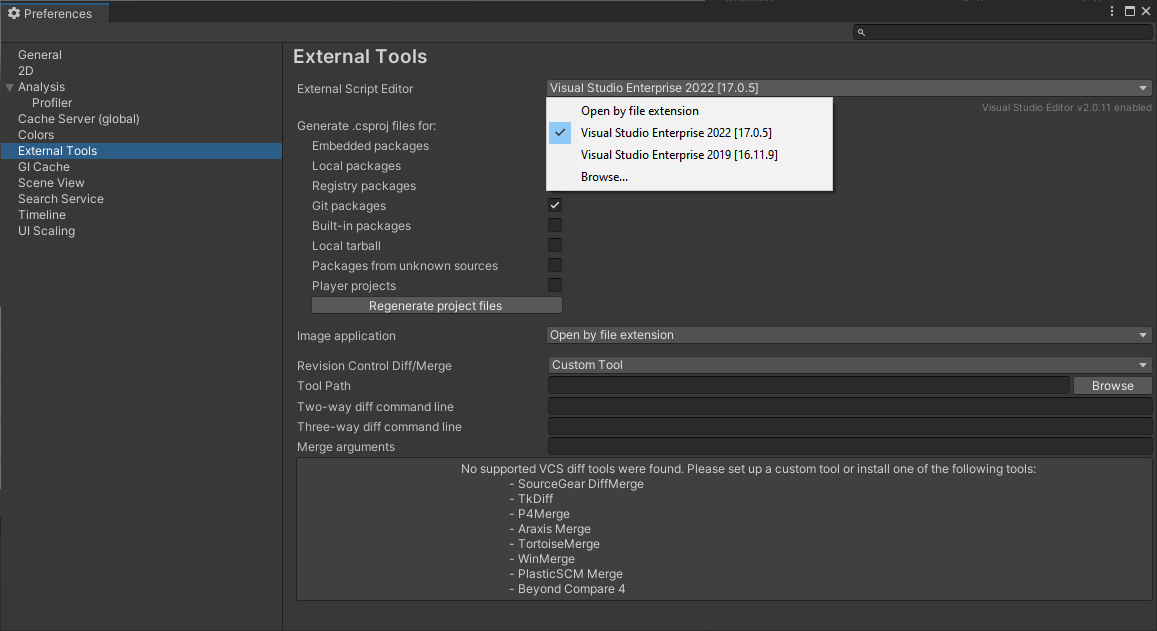
\includegraphics[width=0.8\linewidth]{../../imgs/unity_param_exttools}
\end{center}
		\end{itemize}
	\end{block}
\end{frame}

\begin{frame}[fragile]{Composant script}
	\vfill
	\begin{alertblock}{Attention!}
		Tous les composants scripts héritent de MonoBehaviour! Elle possède pleins de fonction en accord avec son cycle de vie:
		\begin{itemize}
			\item Awake: lorsque le script est chargé pour la première fois.
			\item Start: lorsque le script est lancé pour la première fois.
			\item Update: callback appelé à chaque frame (plusieurs variantes). 
			\item (détail: \url{https://docs.unity3d.com/Manual/ExecutionOrder.html})
		\end{itemize}
	\end{alertblock}

	\vfill
	\begin{block}{Paramétrage de script}
		Les variables publiques sont reconnaissables par l'éditeur et manipulable directement dans l'éditeur. 
	\end{block}
	\vfill
\end{frame}


\begin{frame}{Demo3}
		\vfill
	\begin{block}{Objectifs}
		\begin{itemize}
			\item Dans une scène, ajoutez un cube/sphère.
			\item Ajoutez un nouveau script composant nommé: JeTourne.
			\item Editez le script pour qu'il affiche un message de débogage pour certaines fonctions du cycle de vie et qu'il réalise une rotation autour de lui.
			\item Dans le script faite une rotation de 5° autour de y par frame. Observez.
			\item Modifiez pour que cela se fasse dans \texttt{FixedUpdate} (avec \texttt{Time.fixedDeltaTime}). Observez.
			\item Réalisez un schéma du système Soleil-Terre-Lune qui tourne autour d'eux et entraine l'objet gravitant avec eux d'un point de vue hiérarchique (aucune importance de la véracité physique).
			\item Modifiez le script pour avoir un attribut publique qui correspond à la vitesse de rotation.
		\end{itemize}
	\end{block}
		\vfill
	
\end{frame}



\section{Présentation des interfaces UI}

\begin{frame}{Les interfaces}
	\vfill
	\begin{alertblock}{Attention!}
		Il existe plusieurs kits d'interface graphiques en Unity:
		
\begin{center}
	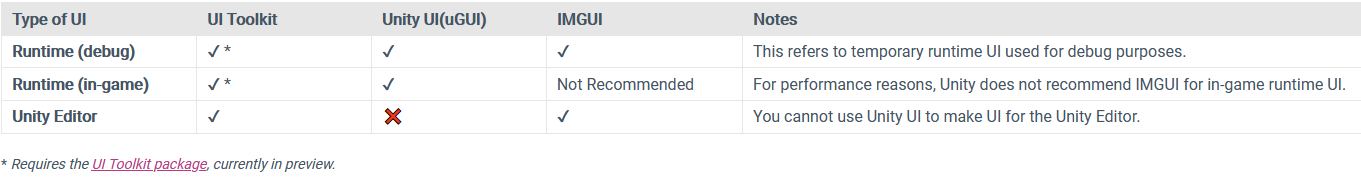
\includegraphics[width=\linewidth]{../../imgs/unity_kits_UI}
\end{center}

		Dans ce cours, nous ferons que du \texttt{Unity UI} qui suit les mécaniques des \texttt{GameObject}. Cependant, il est impossible d'étendre l'éditeur.
	\end{alertblock}
	\vfill
	
		\begin{alertblock}{La zone d'interface se compose }
			Lorsque vous réalisez une interface il est OBLIGATOIRE d'avoir les éléments suivants (Unity peut vous les créer si besoin):
			\begin{itemize}
				\item Canvas: la zone de dessin qui est la base de toute interface (cf démo)
				\item EventSystem: un objet faisant le pont avec les entrées (clavier, souris, \ldots).
			\end{itemize}
		\end{alertblock}
	

	\vfill
\end{frame}

\begin{frame}{Les interfaces}
	\vfill
\begin{block}{Dans ce cours}
	Nous construirons nos widgets graphiques par composition d'élements existant et de script pour compenser des manques.
\end{block}
\vfill
\begin{block}{Spécificité des widgets graphiques}
	Les widgets graphiques n'ont pas de \texttt{Transform} qui gère la position dans la scène, mais un \texttt{RectTransform} qui s'occupe du placement dans le canevas. Le paramétrage est différent.
\end{block}
\vfill

%\begin{block}{Les modes de rendu du Canvas}
%	Un canevas a 3 modes de rendu:
%	\begin{itemize}
%		\item Screen space - Overlay: qui est mode intuitif 2D comme on connait.
%		\item Screen space - Camera: qui subit les modifications de la caméra (comme la perspective)
%		\item World Space: qui place le canevas dans l'environnement 3D.
%	\end{itemize}
%\end{block}

\end{frame}


\begin{frame}{Demo}
	\vfill
	\begin{block}{Objectifs}
		\begin{itemize}
			\item Dans la scène précédente (Soleil-Terre-Lune).
			\item Ajoutez bouton comme interface.
			\item Ajoutez dans le script JeTourne une fonction toggle qui active et désactive la rotation.
			\item Lié le bouton ajouter à la fonction précédente pour contrôler l'animation sur un objet.
			\item Vous pouvez ajouter d'autre bouton pour contrôler les rotations des autres astres.
		\end{itemize}
	\end{block}
	\vfill
	
\end{frame}

\section{La mise en page}

\begin{frame}{La mise en page}
	\begin{alertblock}{Attention!}
Le canevas a toujours une taille précise (dans les paramètres de l'application) et mise à l'échelle. Elle sera donc toujours comme vous la voyez dans l'éditeur!

La mise en page des widgets n'est pas aussi intuitive que les autres outils, en raison de la consommation des replacements.
		
	\end{alertblock}

\begin{block}{Les ancres}
	Tous les widgets ont des ancres qui permettent de fixer leur position au sein de leur parent. 
\end{block}

\hfill
	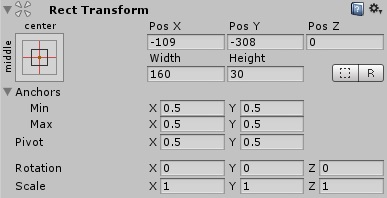
\includegraphics[width=0.45\linewidth]{../../imgs/UI_RectTransform}
\hfill
	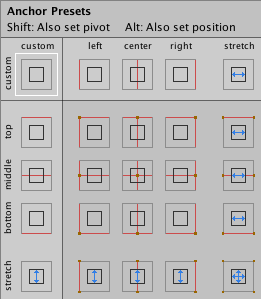
\includegraphics[width=0.25\linewidth]{../../imgs/UI_AnchorPreset}
\hfill


\end{frame}

\section{Petites astuces diverses et autres informations}

\begin{frame}{En Vrac}
\begin{itemize}
	\item L'asset store est strictement interdit dans vos projets (rend les corrections trop compliqués, donc ZERO si dépendance manquante sur nos machines).
	\item Notion de Préfabs et création dynamique.
	\item Mécanisme d'export.
	\item Prudence Git et soumission de vos projets.
	\item Mécanique des inputs (attention refonte dans Unity).
	\item Retrouver un objet? (En TP)
	\item Faire plusieurs scènes pour expérimenter.
\end{itemize}
\end{frame}


  
%%% Local Variables: 
%%% mode: latex
%%% TeX-master: "Cours1"
%%% End: 

\end{document}